%***************************************PREAMBLE***************************************
\documentclass[a4paper,12pt]{article}

\usepackage{arxiv}

\usepackage[utf8]{inputenc} % allow utf-8 input
\usepackage[T1]{fontenc}    % use 8-bit T1 fonts
\usepackage{hyperref}       % hyperlinks
\usepackage{url}            % simple URL typesetting
\usepackage{booktabs}       % professional-quality tables
\usepackage{amsfonts}       % blackboard math symbols
\usepackage{nicefrac}       % compact symbols for 1/2, etc.
\usepackage{microtype}      % microtypography
\usepackage{lipsum}
\usepackage{float}

\usepackage[utf8]{inputenc}
\usepackage{graphicx}
\usepackage{setspace}
\usepackage{tgtermes}

\title{Beat the Bookie}

\author
{
 Group Name: \texttt{Group I}\\
  Department of Electronic and Electrical Engineering\\
  University College London\\
  London, WC1E 6BT\\
}

\date{7\textsuperscript{th} January 2019}

\graphicspath{ {./images/} }

%***************************************DOCUMENT***************************************
\begin{document}

\maketitle

\section{Introduction}

The aim of this project is to utilize past match data to make a prediction for the result of a match in the future. We will not be predicting the exact score; Instead we will be predicting if the Home team wins (“H”), the away team wins (“A”) or the game ends as a draw (“D”). The league that we will be concerned with the English Premier League (EPL).\\
\\
In each season of the EPL 20 domestic teams compete. For each matching, two games will be played: one at each of the two teams’ home stadiums. This will result in a team always being the “home” team and the other being the “away” team.  

\section{Data Transformation and Exploration}

	The raw match data that was provided to us in the form of a csv file was imported and analysed thoroughly to identify any patterns and trends that could be exploited. Furthermore, the provided data will be manipulated to calculate metrics that describe the team’s performance. These metrics will act as features in the design matrix and will eventually be used to train the classifier model. 
	
	\subsection{Columns of the Provided Dataset }
	
		The provided dataset contained 22 columns. It contained data of all EPL matches from 2008 to 2019. Table 2.1 lists the columns of the provided dataset and a brief explanation as to what each quantity represents.
	
	\subsection{Number of Matches}
	
		The first thing that was observed was the number of matches played by each of the teams. It was identified that not all the teams played the same number of games from 2008 to 2019. This is most likely due to some teams getting relegated (dropping out of the EPL) and other teams being promoted (joining the EPL). This will result in the consistently strong teams who have remained in the EPL throughout having played the most games while those that have been relegated and promoted having played less games in the dataset. This is clearly visible from Fig. 2.1. The 7 teams with the most matches have played the same number of matches and are likely to have been consistently in the EPL throughout the 2008-2019 time period.  
		
		\begin{figure}[H]
%			\renewcommand\thefigure{2.1}
			\centering
			
			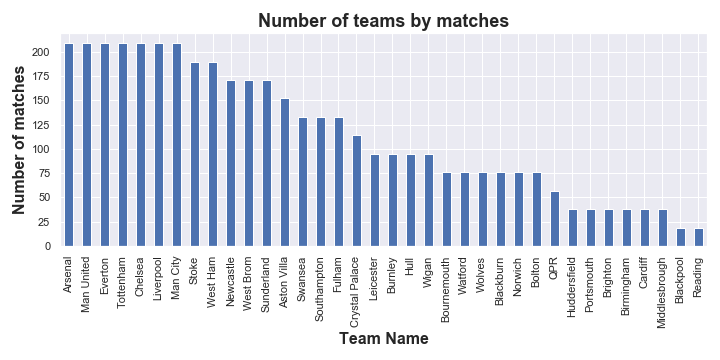
\includegraphics[scale=0.6]{num_of_matches.png}
			\caption{A count plot of the number of matches played by each of the different teams. It is clearly visible that not all teams played the same number of games.}
		\end{figure}
		
		Another quantity that was confirmed was if all possible pairings have played one another at least once in the time period of the dataset. This was found to be not the case. This is not possible due to relegation and promotion changing the list of competing teams from season to season.  
	
	\subsection{Histogram Plots of Numerical Columns}
		
		From Table 2.1.1 it is evident that most columns are integers. The distribution of each of these columns was investigated by plotting the histogram for each column. In addition to this, each bar in the histogram is split according to the full-time result (FTR). The plots are presented in Fig. 2.2 for each of the 16 integer columns in the provided dataset. It is clearly visible that most of these plots have a clear maximum either side of which the frequency drops. This could possibly indicate that these quantities may be modelled using a Poisson distribution. This is possible as each of the quantities is measured per match and therefore it is measured at a constant rate. This relationship is most clearly visible with datasets that have a large variation (i.e. have a large range). An example is the HS plot. It is clearly visible that this set of data may be modelled with a mean of around 12.\\
		\\
		\textbf{FTHG/FTAG}: The modal number of goals scored in a match by the home team is 1 whereas the modal number of goals scored in a match by the away team is 0. This loosely suggests that a team is likely to perform better at home than away, as expected.\\
		\textbf{HTHG/ HTAG}: The difference between the half time goals scored by home and away teams is a bit more subtle. The modal number of goals is 0 for both and the trends are similar.\\
		\textbf{HS/AS}: The modal class for the home shots is 12 while the modal class for the away shots is 10. This suggests a slightly lower performance when a team plays away compared to at home.\\
		\textbf{HST/AST}: By analysing the plot, the HST graph has a mean of around 4.5 while the AST graph has a mean of around 4. Which once again hints at a better performance at home.\\
		\textbf{HF/AF}: The distribution of fouls committed by the home and away teams seem to be similarly distributed.\\
		\textbf{HC/AC}: The distribution of corners is such that corners occur slightly more \\
		\textbf{HY/AY}: The approximate mean of the away plot is slightly higher than that of the home plot suggesting that teams receive more yellow cards when they play away.\\
		\textbf{HR/AR}: The occurrence of red cards was very rare, and the maximum number of red cards was 1. The histogram plot also suggests that the team that receives a red card is more likely to lose the game
		
		\begin{figure}[H]
%			\renewcommand\thefigure{2.1}
			\centering
			
			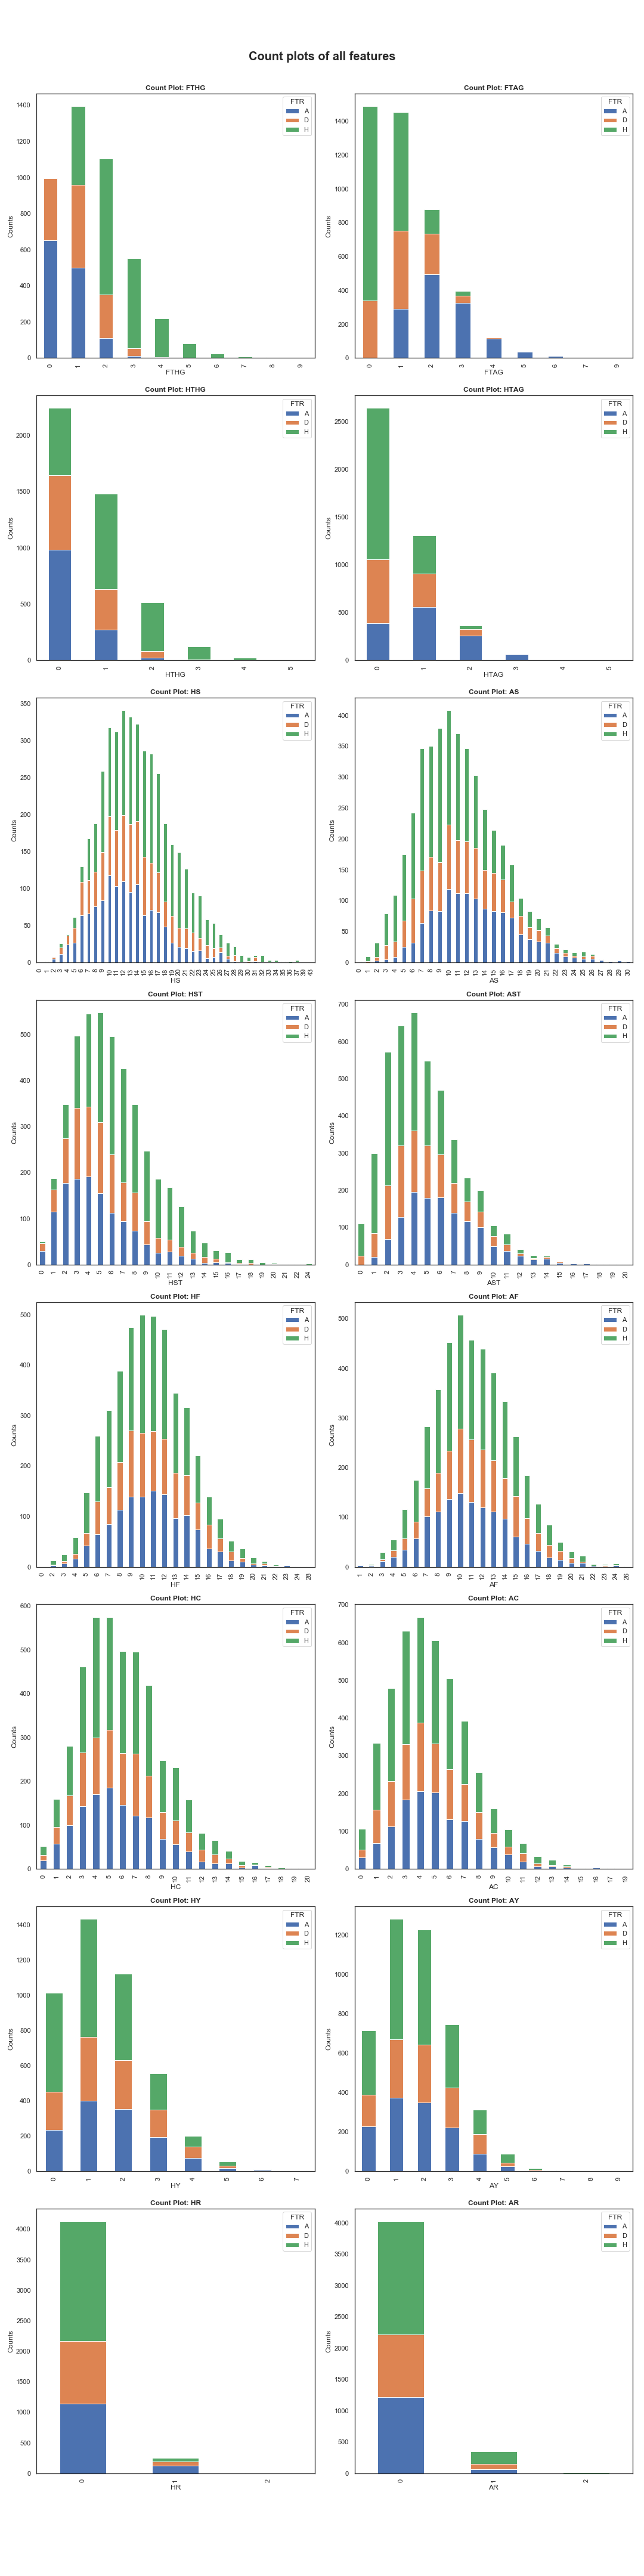
\includegraphics[scale=0.32]{count_plot_all.png}
			\caption{A count plot of the number of matches played by each of the different teams. It is clearly visible that not all teams played the same number of games.}
		\end{figure}
		
	\subsection{Analysis of Non-Numerical Columns}
		
		As shown by table 2.1.1 the non-numerical columns of the dataset are “Date”, “HomeTeam”, “AwayTeam” and “Referee”. There are 36 unique teams listed in the “HomeTeam” and “AwayTeam” columns. As expected, all teams that appear in “HomeTeam” also appear in “AwayTeam” and vice versa. As previously discussed, one season only consists of 20 competing teams. The larger number of teams in the dataset is once again due to the relegation and promotion of teams from season to season.\\
		\\
		There are also 36 unique referees across the dataset. Despite this number being equal to the number of unique teams, this is believed to be a coincidence as no specific rules on the assignment of referees that would result in this was found.\\
		\\
		The “Date” column was analysed and found that matches only occurred in months January to May and August to December. This suggests that a season of the EPL runs from August to May. This can be used to split the dataset by season and thereby find variation in team statistics by season.  
	
	\subsection{Investigation of variation in data}
	
		To investigate the spread of the data, we observe the box-plot for each of the columns containing numerical data. This is shown in fig X.
		
		\begin{figure}[H]
%			\renewcommand\thefigure{2.1}
			\centering
			
			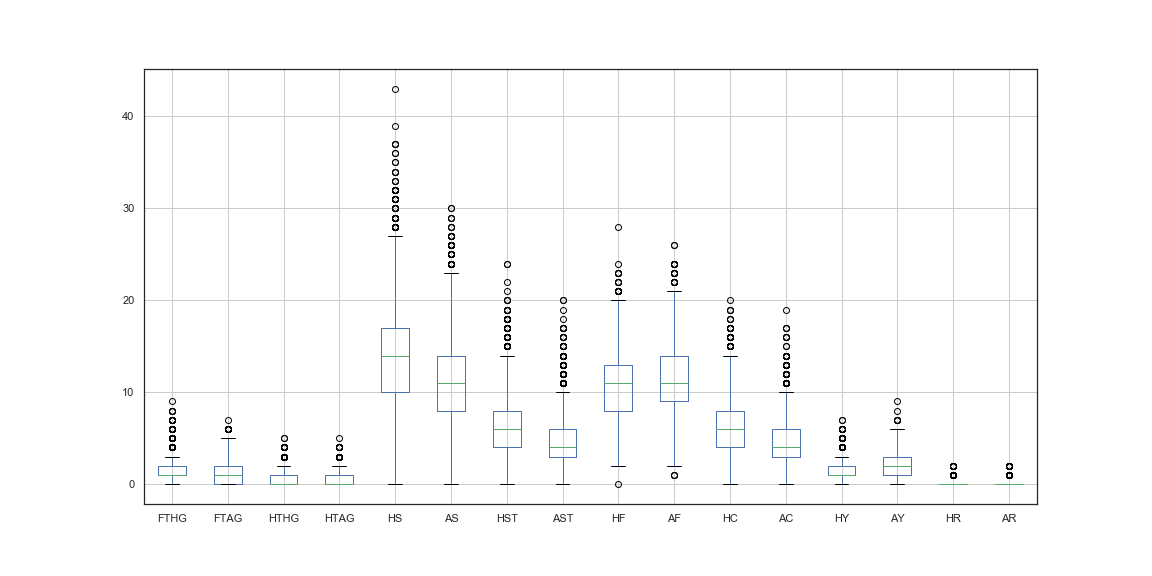
\includegraphics[scale=0.32]{raw_box_plot.png}
			\caption{A count plot of the number of matches played by each of the different teams. It is clearly visible that not all teams played the same number of games.}
		\end{figure}
	
	\subsection{Correlation between columns of raw match data }
	
		To analyse the patterns in the dataset, the correlation between each of the columns was calculated. This data was represented by using a heatmap. The colours of the cells correspond to the Pearson correlation coefficient between the two columns. The most distinct feature of this heatmap is the diagonal representing correlations of 1.0. This is due to the correlation of each of the features with itself. It also follows from this that this correlation matrix is symmetrical.\\
		\\
		The half time home goals (HTHG) is strongly correlated with the full-time home goals (FTHG) with a correlation of 0.7. This also applies to the away case (HTAG and FTAG). The other strongly correlated columns are the half time result and full-time result columns (HTR and FTR). This strong correlation implies that the team that was winning at half time is likely to win the whole match as well.\\
		\\
		Another interesting correlation is that between the home corners (HC) and home shots (HS) with a correlation of 0.5. This suggests that some corners result in attempted shots at the goal for the team. Furthermore, HC also correlates with shots on target (HST) with a score of 0.4 suggesting that corners also result in shots on the target. The same applies to the away team (HC, AS and AST). However, at away matches, the correlation between AC and AST is 0.3 as opposed to 0.4 at home suggesting that corners are less likely to lead to shots on the target when a team plays away.\\
		\\
		A more obvious correlation is that the home fouls (HF) correlates with the number of yellow cards received by the home team (HY). This can easily be explained by the fact that aggressive/dangerous fouls often lead to yellow cards.\\
		\\
		It is also clearly visible that the referee column has no correlation with any of the other columns, which is indicative that it is chosen at random and does not influence the performance of either team. This relationship is expected as the job of a referee is to preside of the game from neutral point without being biased to either team.
		
		\begin{figure}[H]
%			\renewcommand\thefigure{2.1}
			\centering
			
			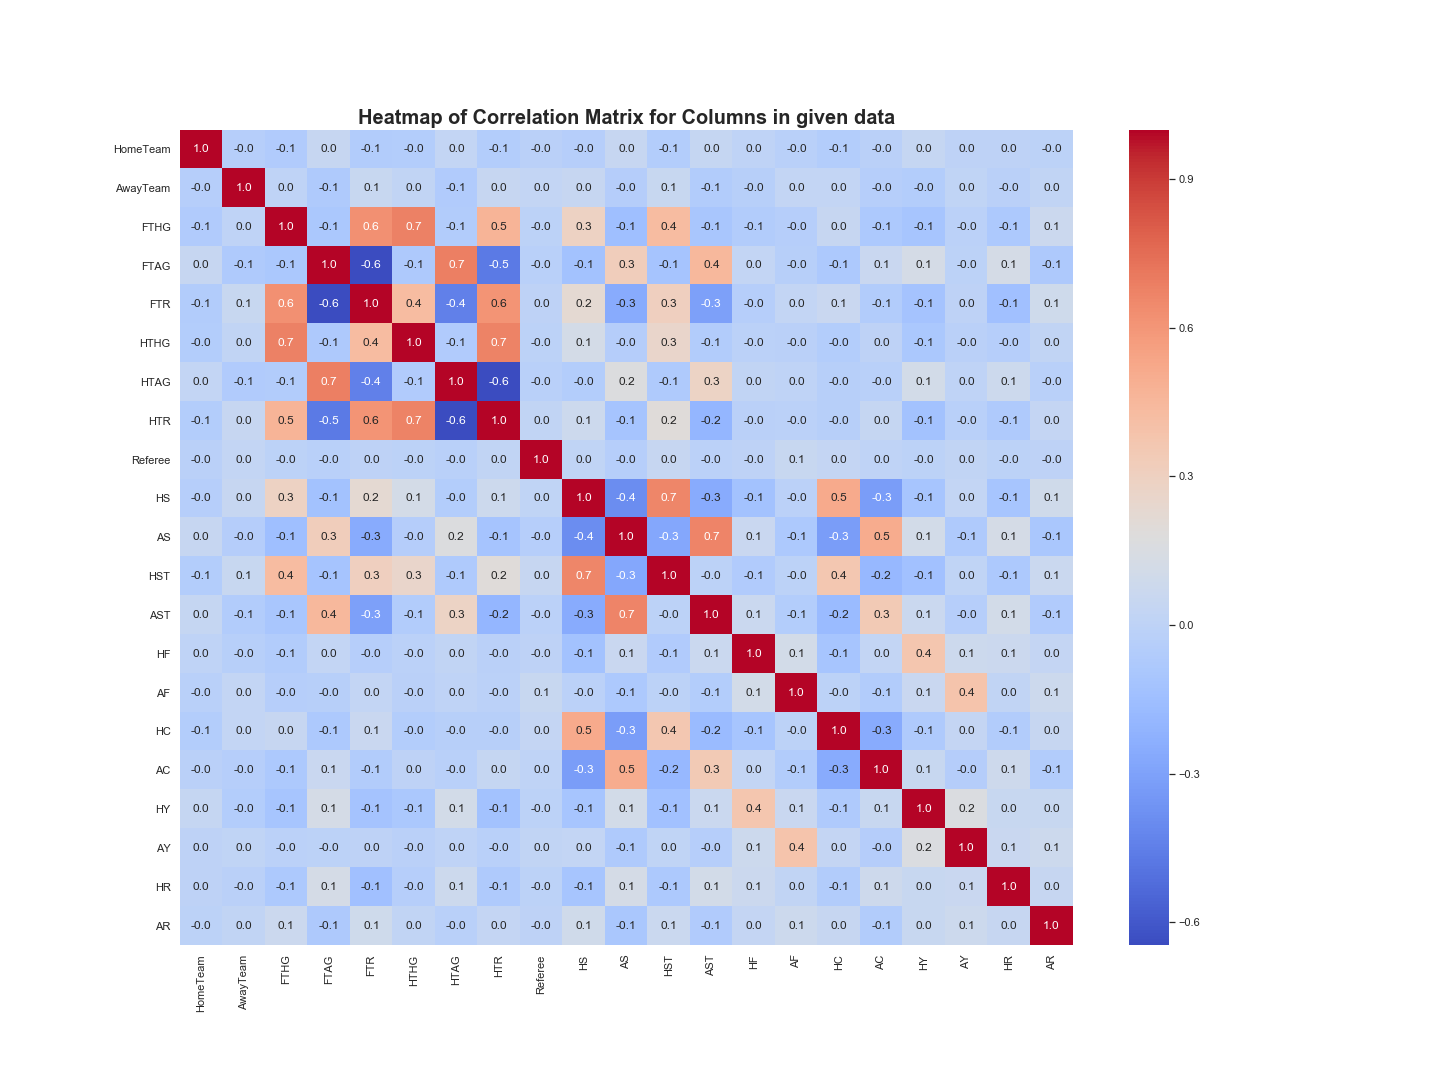
\includegraphics[scale=0.4]{raw_corr_heatmap.png}
			\caption{A count plot of the number of matches played by each of the different teams. It is clearly visible that not all teams played the same number of games.}
		\end{figure}
		
	
	
	
\section{Methodology Overview}

\section{Model Training \& Validation}

\section{Results}

\section{Final predictions on Test Set}

\section{Conclusion}

\end{document}
